\section{Results}
\setlength{\parindent}{10ex}

This section contains the results for each model observed by this work.
Including results for the regression, classification, and novel grid optimized model.
Each section includes figures representing the metric scores.

\subsection{Regression Results}
Regression \ac{ML} models were fit in order to compare to existing physics models.
Three models were fit to the data: 
an SVM regression model, a Naive Bayes regression model, and a simple linear regression model.
These models were trained against a reduced set of data shown in figure \ref{fig:trainset}, and validated against the world wide data not used in the training phase.
Each model was fit against selected features from the Genetic Algorithm feature selector.
The \(R^2\) score for each model can be found in figure \ref{fig:r2_barplot_regression}.
The RMSE of each model can be found in figure \ref{fig:rmse_barplot_regression}.



\begin{figure}[h]
    \centering
    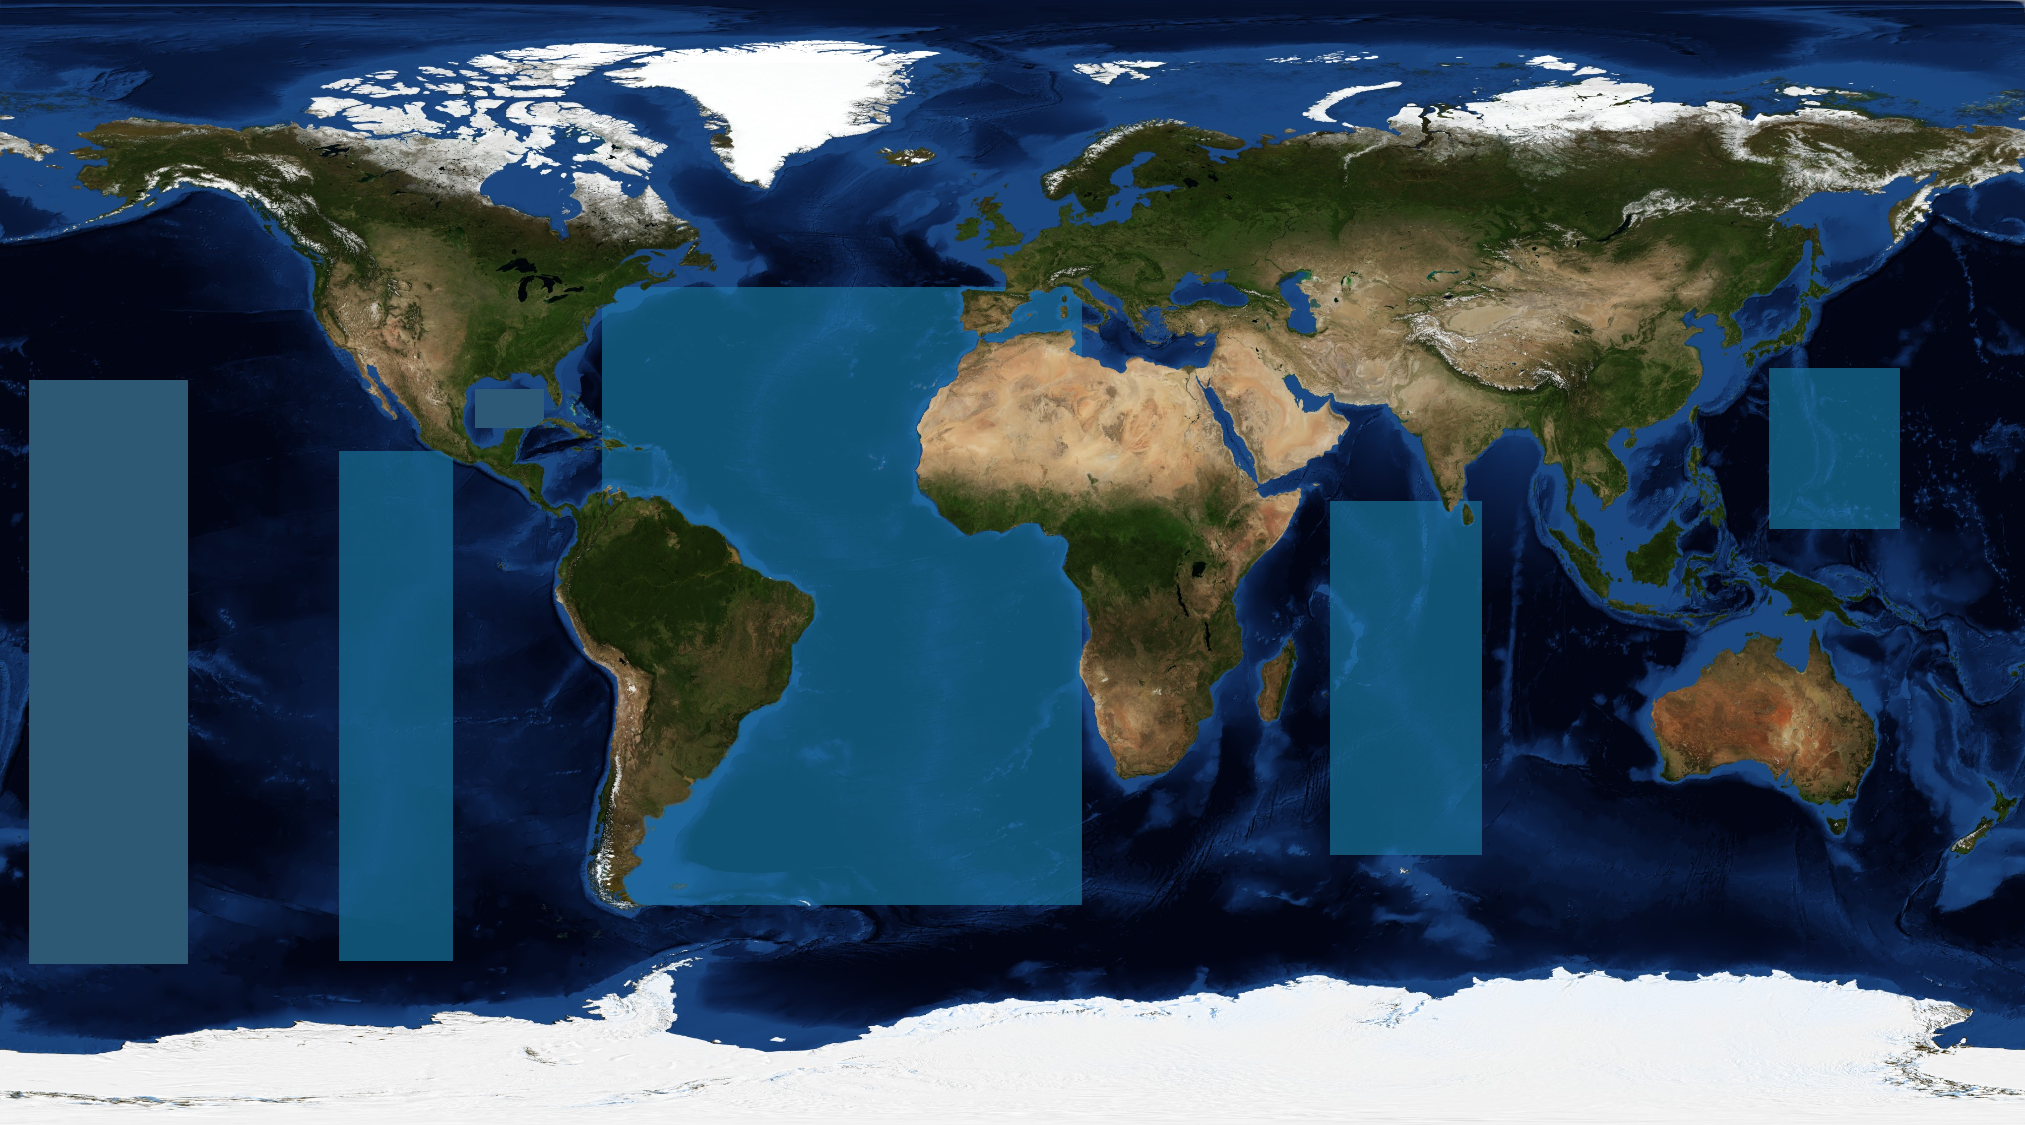
\includegraphics[width=\textwidth]{worldtraininglocal.png}
    \caption{Figure demonstrating initial training sets for regression. These sets were selected for training and testing was performed against the rest of the world.}
    \label{fig:trainset}
\end{figure}

% \begin{table}[htb]
%     \centering
%     \begin{tabular}{|c c c|}
%         \hline
% 		\textbf{Model} & \textbf{\(R^2\)} & \textbf{RMSE} \\
% 		\hline
% 		SVM Regression & 0.841 & 365.23m \\
% 		Naive Bayes & 0.884 & 294.92m \\
%         Linear Regression & 0.885 & 265.43m \\
% 	    \hline
%     \end{tabular}
%     \label{table:REGRESSION_RESULTS}
%     \caption{Regression Results}
% \end{table}

\begin{figure}[h]
    \centering
    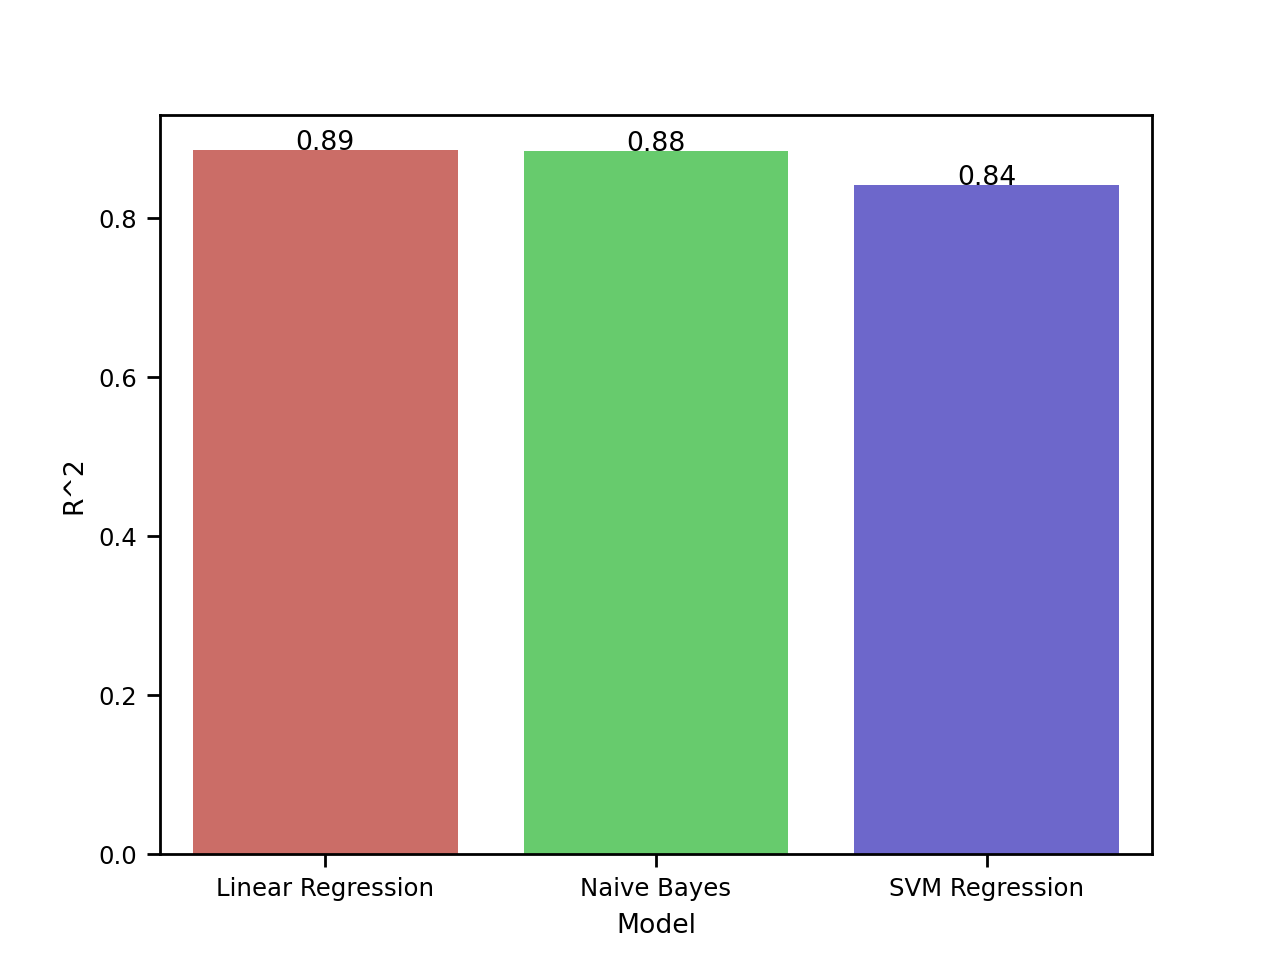
\includegraphics[width=\textwidth]{rsquared_barplot_regression.png}
    \caption{Bar chart showing \(R^2\) score for each model}
    \label{fig:r2_barplot_regression}
\end{figure}

\begin{figure}[h]
    \centering
    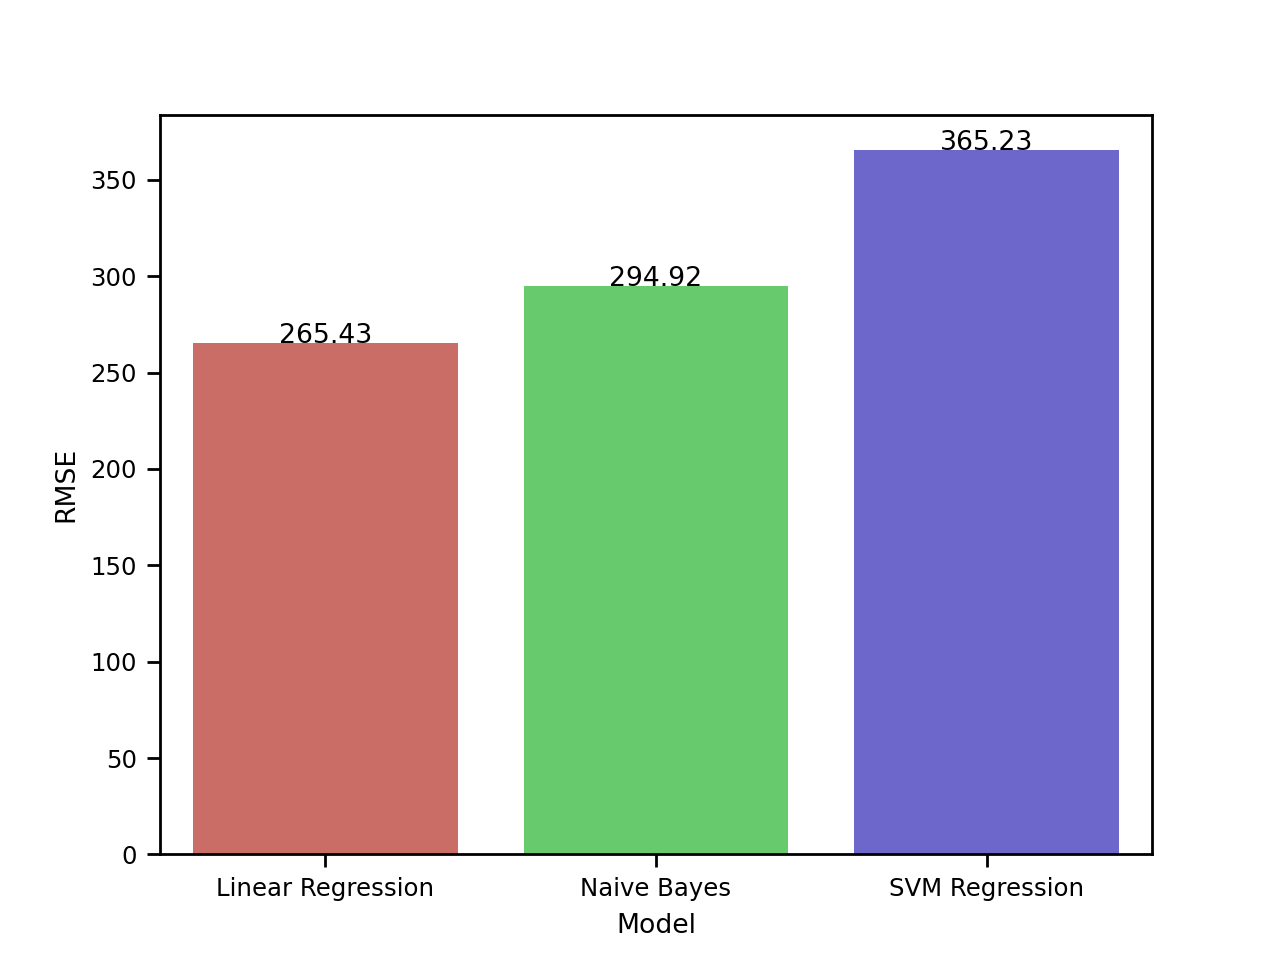
\includegraphics[width=\textwidth]{rmse_bar_regression.png} 
    \caption{Bar chart showing RMSE for each model}
    \label{fig:rmse_barplot_regression}
\end{figure}

% \subsubsection{Regression Results Discussion}
% \cite{jena2012prediction} achieved a \ac{RMSE} of \~{}175m in their optimized model.
% The linear regression model I fit is 100 meters less accurate than the optimized model used in \cite{jena2012prediction}.
% However, the purpose of the test is not to achieve accurate predictions, but to identify if \ac{ML} models can be viable.
% Therefore, the accuracy of these models is less important than identifying the viability of the models.
% The training data used is essentially predicted bathymetry, but shows that fitting a model to true bathymetry will yield a similar result.
% Analyizing the \(R^2\) score gives evidence of the viability of the model.
% This score suggests that there are underlying relationships in the model that can be used to train a successful model.

\subsection{Classification Results}
\setlength{\parindent}{10ex}
%Maybe reword this opening chapter???
To facilitate classification, trained models need to predict discrete values instead of continuous values.
This conversion was executed by mapping the bathymetry values into discrete classes.
This conversion proved to be trivial because of the ordered nature of bathymetry.
Classification models are simpler and easier to fit than regression models.
Ideally, the decision surfaces will benefit from the conversion and yield better results.
This makes it difficult to compare directly to the error reported in existing physics models.
A set of metrics including: precision, recall, f1 score, and balanced accuracy were used to analyze the viability of the models.

\par
The ordinal classes were binned on a interval of 150 meters.
This was done to easily compare accuracy to model in \cite{jena2012prediction}.
Validation was preformed using a 10 fold cross validation using balanced accuracy as the scoring function.
The F1 results for each model can be found in figure \ref{fig:f1_barplot_classification}.
The Balanced Accuracy for each model can be found in figure \ref{fig:balacc_barplot_classification}.

\par
The Decision Tree classifier performed significantly worse than the other models.
The 47\% balanced accuracy is not usable for predictions.
Potentially, parameter tuning, and maybe feature selection could improve this model.

% \begin{table}[htb]
%     \centering
%     \begin{tabular}{|c c c|}
%         \hline
% 		\textbf{Model} & \textbf{Average F1 Score} & \textbf{Mean Balanced Accuracy} \\
% 		\hline
% 		Random Forest & 0.81 & 0.82 \\
%         Bagging & 0.80 & 0.79 \\
%         Decision Tree & 0.44 & 0.47 \\
%         \hline
%     \end{tabular}
%     \label{table:CLASSIFICATION_RESULTS}
%     \caption{Classification Results}
% \end{table}

\begin{figure}[h]
    \centering
    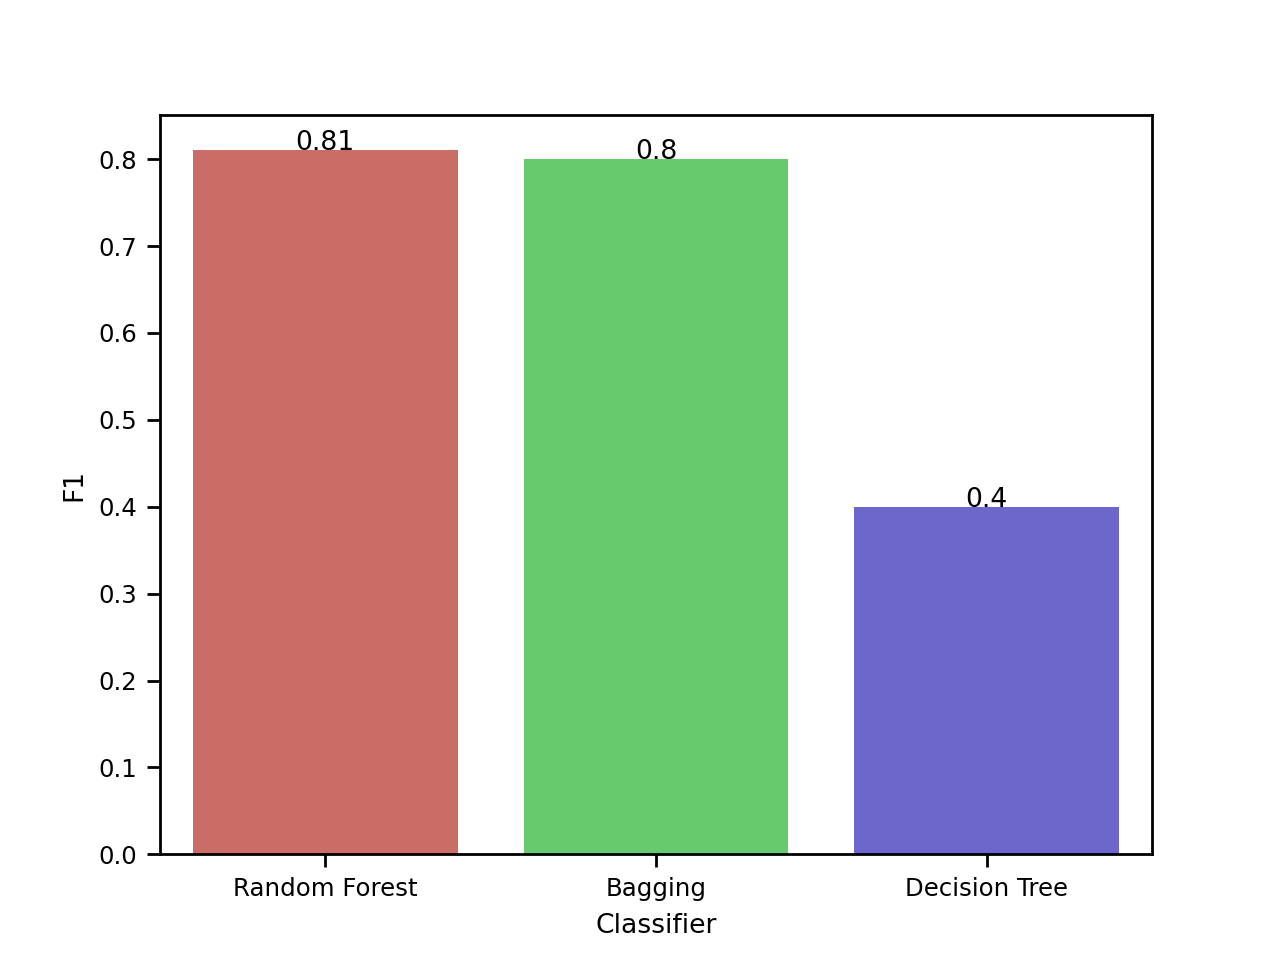
\includegraphics[width=\textwidth]{f1_bar_classification.png}
    \caption{Bar chart showing F1 score for each classifier}
    \label{fig:f1_barplot_classification}
\end{figure}

\begin{figure}[h]
    \centering
    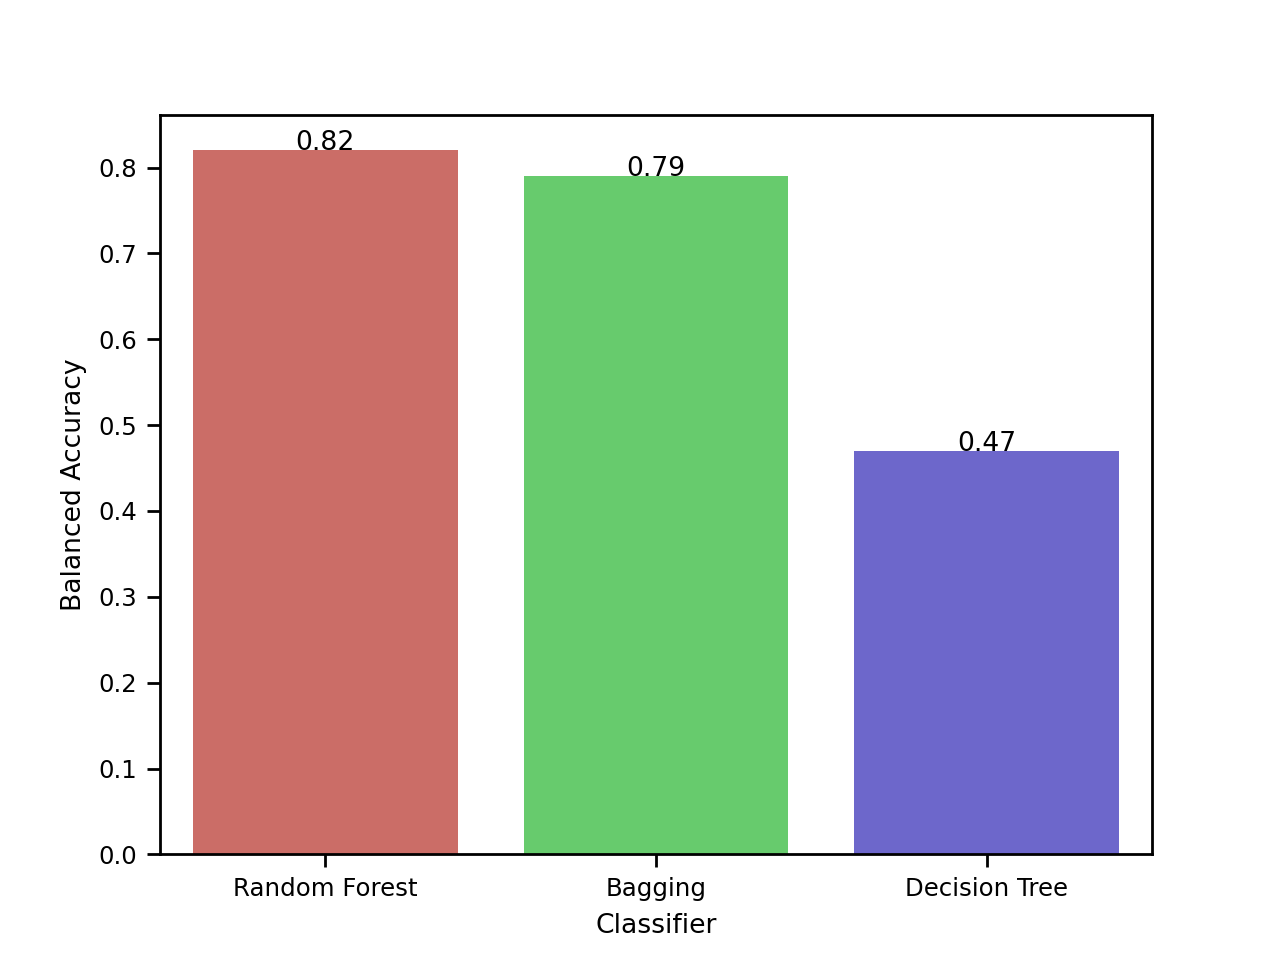
\includegraphics[width=\textwidth]{balacc_bar_classification.png}
    \caption{Bar chart showing balanced accuracy for each classifier}
    \label{fig:balacc_barplot_classification}
\end{figure}

\subsection{Optimized Grid Model}
\setlength{\parindent}{10ex}
%Purpose of this section is to identify the optimized grid structure.
%I need to check with Hoque to identify what I should and shouldnt include
%I need to consider rewording this and restructuring to manage the correctness for example etc.
% Further analysis of figure \ref{fig:rfc_report} shows that models are sensitive to potentially local characteristics.
% In an attempt to test this notion and increase the accuracy of these models a novel model selection method was employed.
% The objective being to identify if a model will predict more accuractly based on geospatial location.
% The hypothysis being that decision boundaries across different models will respond to features based on location.

The Grid Optimized Model Injector Classifier is concerned with testing the best model fit hypothesis.
The theory being that there is not a best fit model for predicting bathymetry across the Earth.
For example, a model may be excellent at predicting shallow bathymetry where there is a particular feature that is sensitive to a sediment type.
Where as, another model may be excellent at predicting bathymetry in deep water scenarios.
This novel Grid Optimized Model Injector tests this theory by implementing a model that optimizes by geospatial location.

\begin{figure}[h]
    \centering
    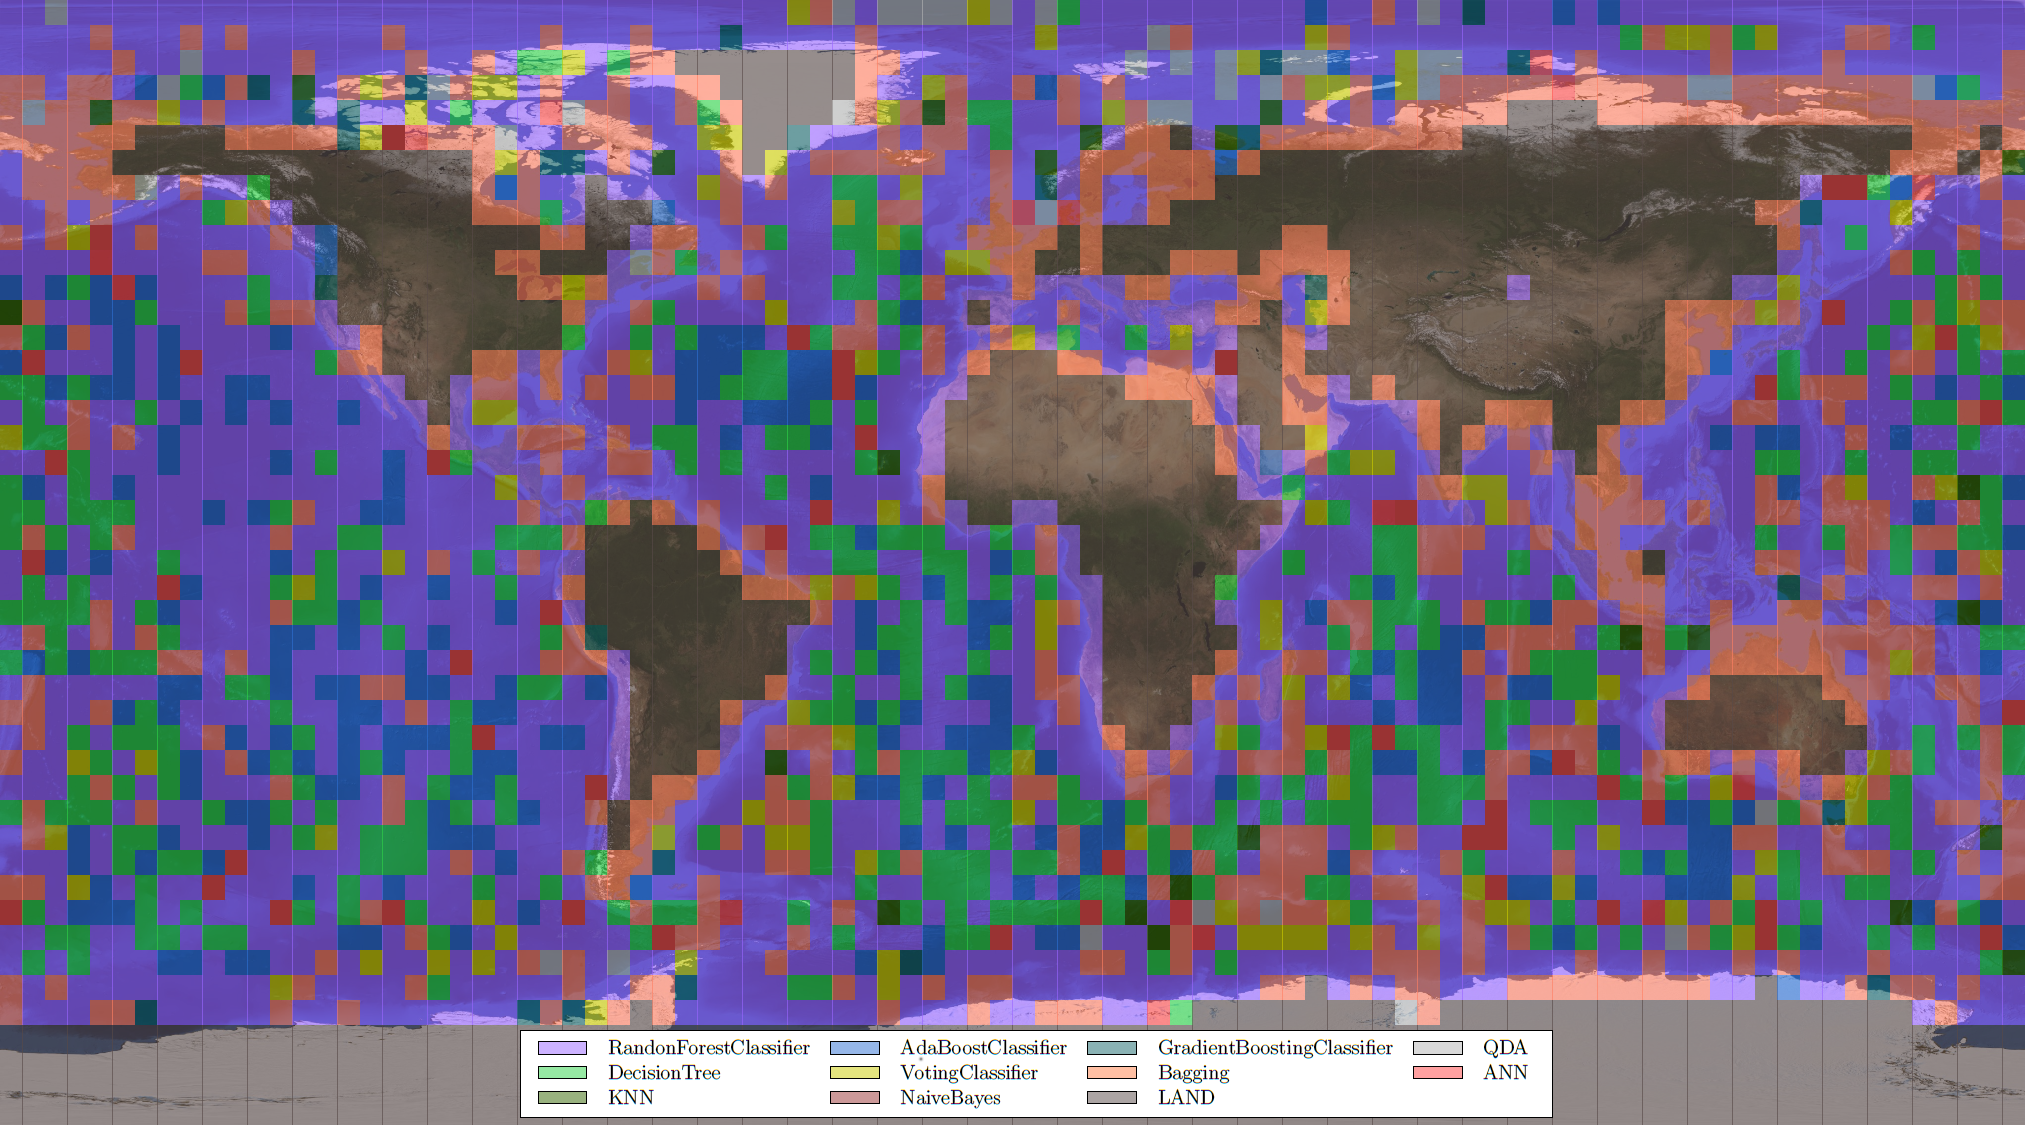
\includegraphics[width=\textwidth]{optgriddraft.png}
    \caption{Graphic Showing the World Coverages and Successful Models.
    Each square represents a coverage.
    The shaded color represents the model that was most successful in that coverage.}
    \label{fig:coveragegrid}
\end{figure}

%Give the background for the idea in this section!
\subsection{Analysis of Global Model Optimization}
This hypothesis was tested by building a model that optimizes by geospatial location.
In order to optimize by location a cache of "best fit" models for each location needed to be created.
This can be performed by comparing the performance of a set of models for predicting every point in a grid.
However, this can take an extremely long time because of the size of these geospatial grids.
To simplify this experiment, for sake of time and computing resources, the world was instead split into N coverages.
These coverages represent an area of the Earth and will suffice for the experiment of comparing model performance across geospatial locations.
The performance of a set of models for each coverage was recorded.
The best performing model in that coverage was then exported and saved to a map of best fit models to a geospatial bounding box.
The results of this experiment are displayed in figure \ref{fig:coveragegrid}.

\begin{figure}[h]
    \centering
    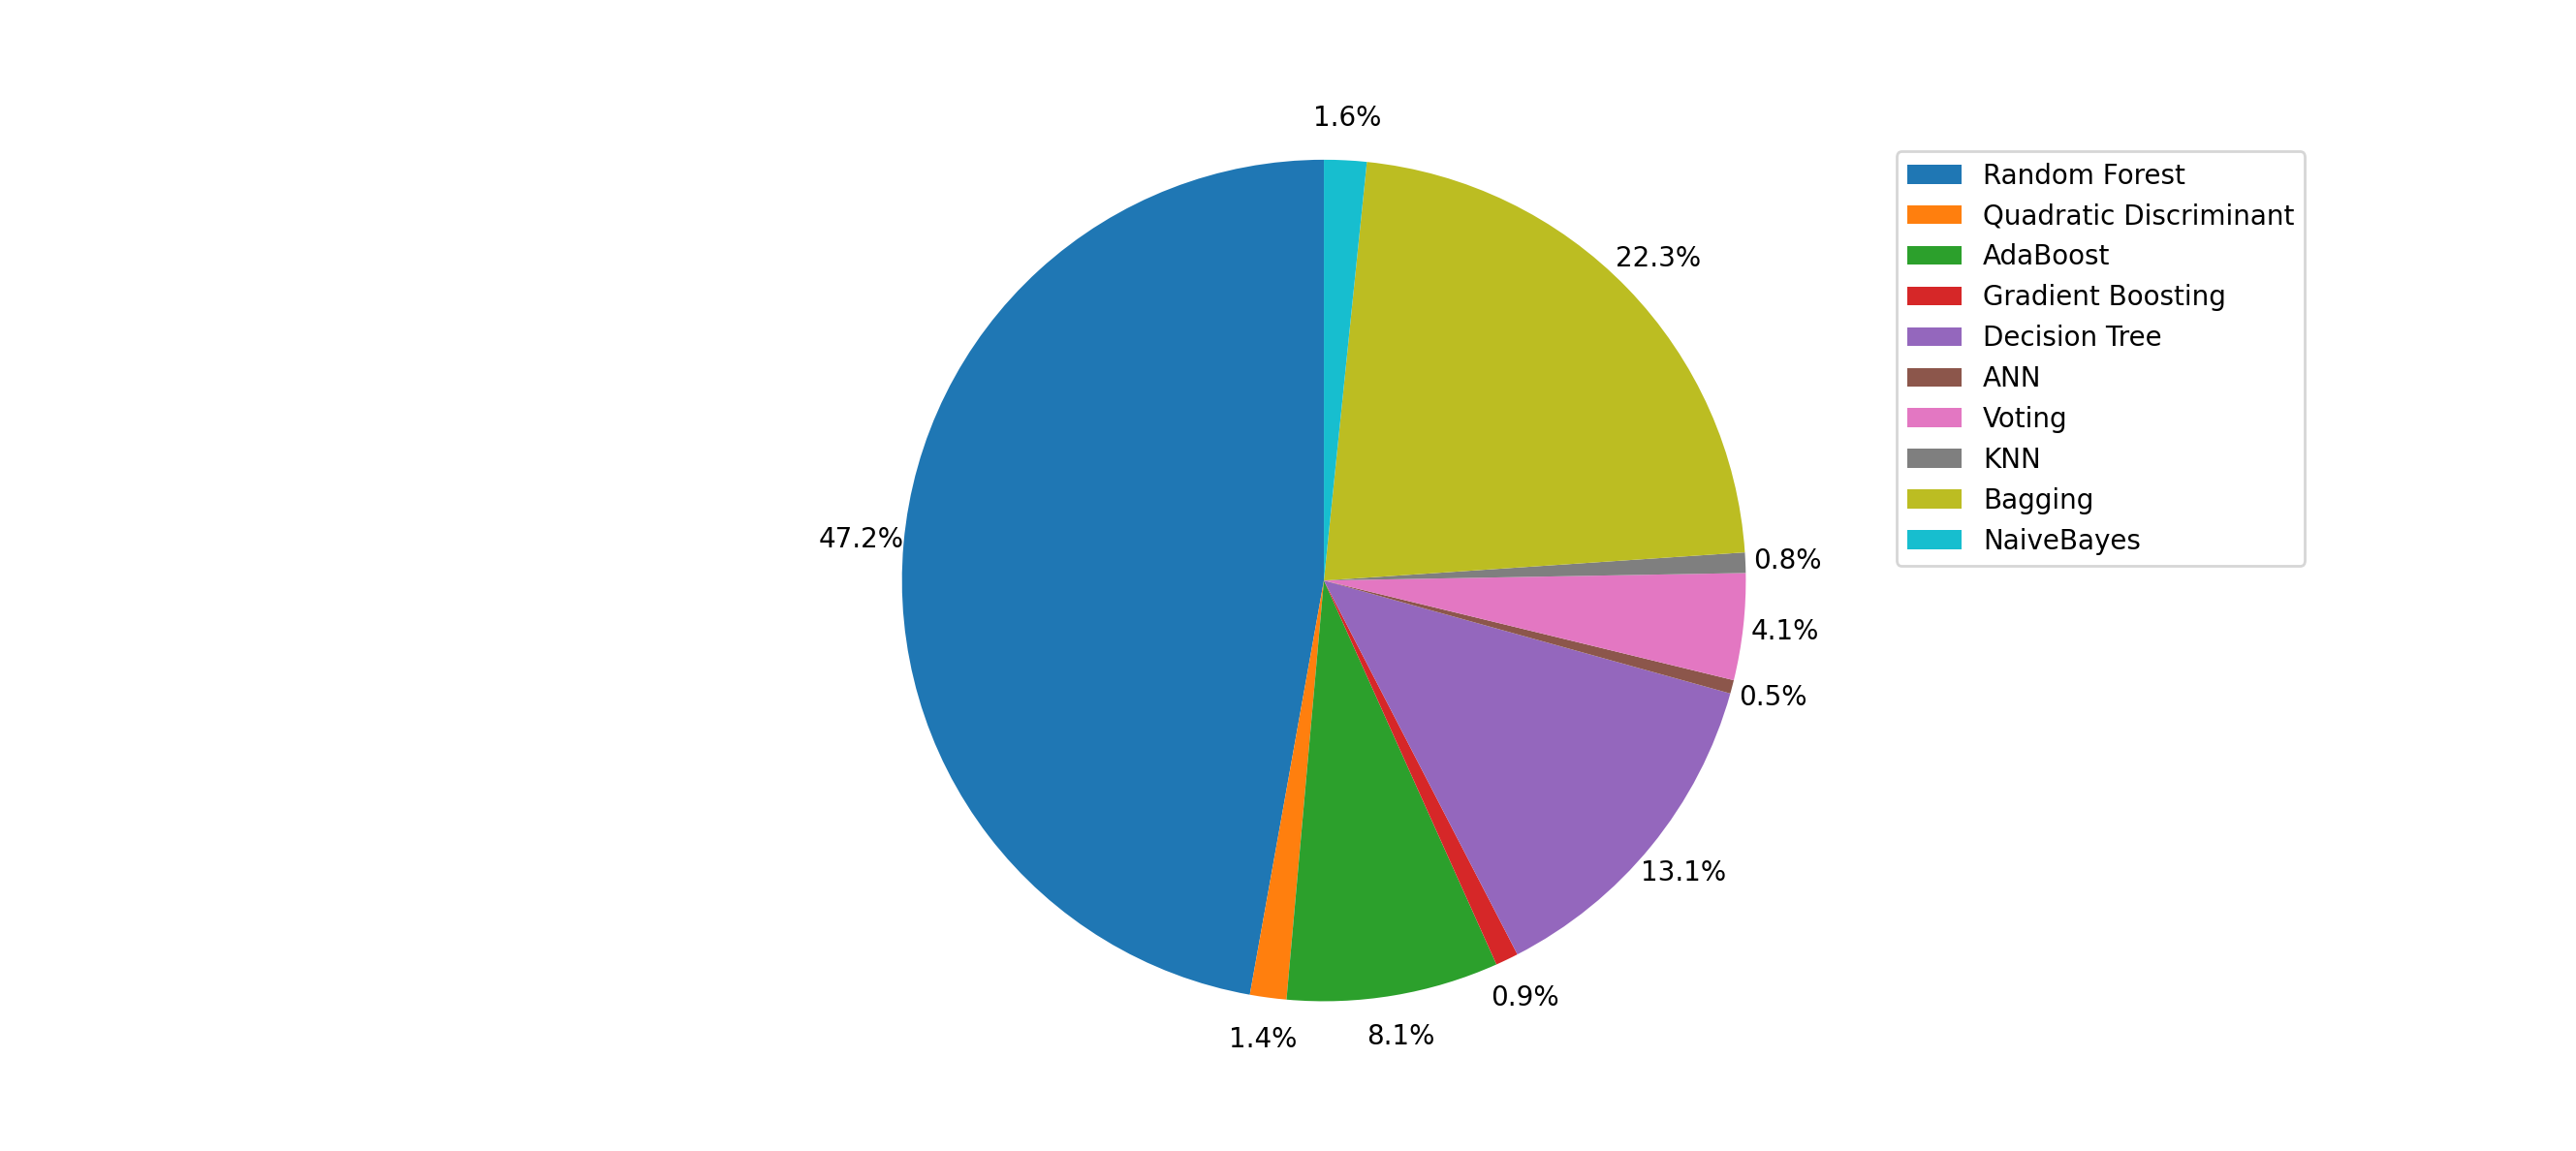
\includegraphics[width=\textwidth]{best_fit_percentage.png}
    \caption{Pie plot showing the percentage of coverages where a model was "best fit". These percentages represent the number of areas where a model performed the best. 
    The percentage will give an indication of the success of a model.}
    \label{fig:pie_best_fit}
\end{figure}

\par
Figure \ref{fig:coveragegrid} shows several interesting things.
Figure \ref{fig:pie_best_fit} shows the percentage that each model was a best fit.
The random forest classifier was the best fit model for a large portion of the oceans.
On the other hand, the Bagging classifier consistently performed well along the coast lines.
The reasons for why these classifiers may have performed so well in those areas will be touched upon in the discussions section.


\begin{figure}[h]
    \centering
    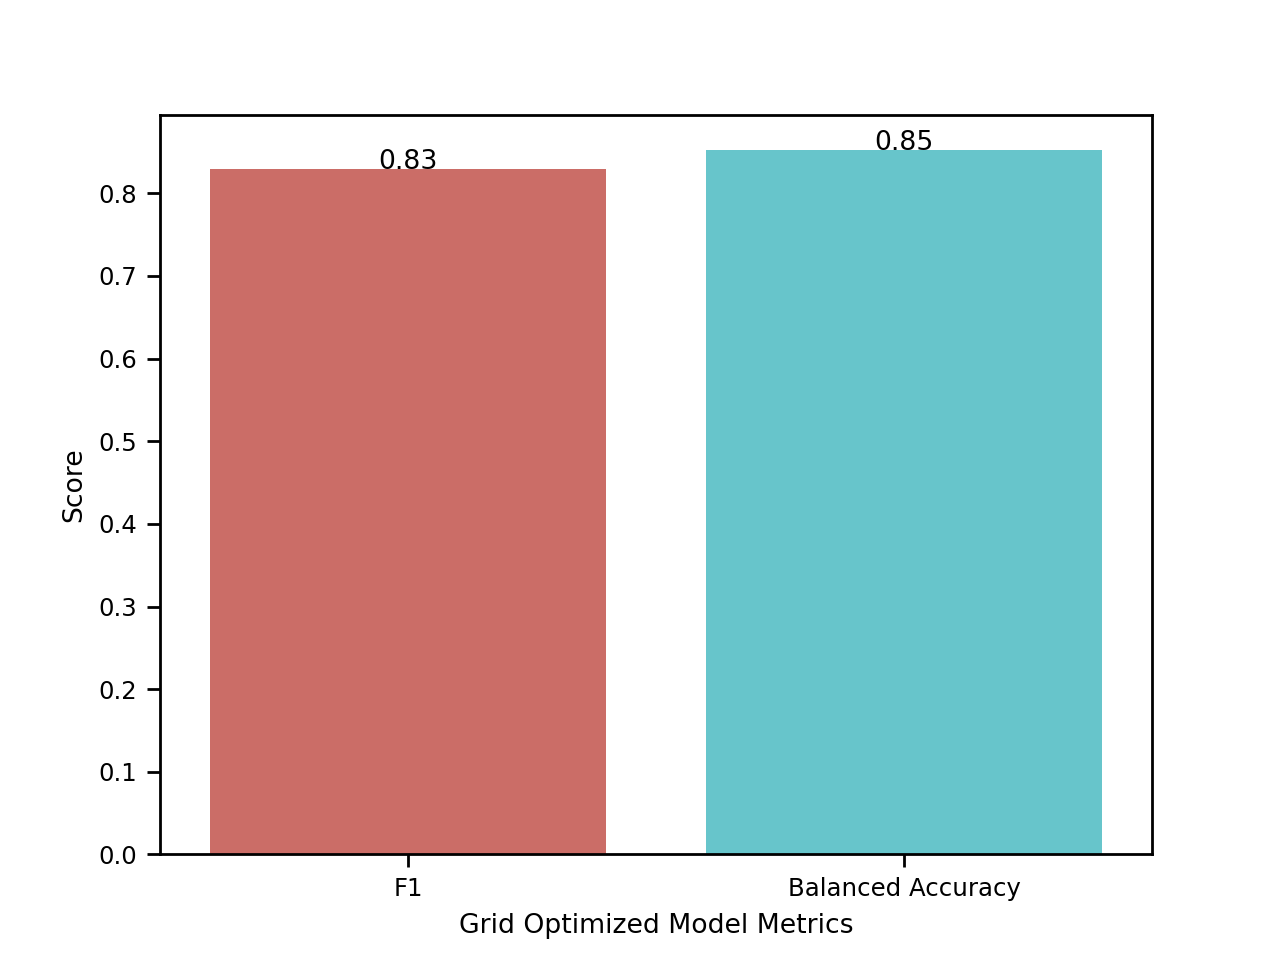
\includegraphics[width=\textwidth]{grid_opt_results.png}
    \caption{Bar chart showing Grid Optimized Model results}
    \label{fig:grid_opt_barplot}
\end{figure}
%In this section I am defining what the Grid optimization is and why it matters.
%There may be a better name for this?? Who knows really...
\subsubsection{Grid Optimizing Results}
Using the successful model for each coverage as an \textit{optimum} selection.
The optimum selection improved the prediction accuracy of the model by several percent.
See figure \ref{fig:grid_opt_barplot} for the results of the model.


